\documentclass[aspectratio=169]{ctexbeamer}
\definecolor{urls}{RGB}{137, 180, 250}
\definecolor{link_text}{RGB}{245, 224, 220}
\hypersetup{
  colorlinks,
  linkcolor=link_text,
  urlcolor=urls,
}
\renewcommand{\UrlFont}{\ttfamily\scriptsize}

\usetheme{AnnArbor}
\usepackage[style=Mocha,accent=Rosewater]{beamercolorthemecatppuccin}

\usefonttheme{serif}
\usefonttheme{professionalfonts}

\usepackage[T1]{fontenc}
\setmainfont{LXGW WenKai}
% \setmainfont{Cascadia Code NF}
% \setsansfont{}
\setmonofont{Cascadia Code NF}
\usepackage{xeCJK}
\setCJKmainfont{LXGW WenKai}
% \setCJKmainfont{}
\setCJKmonofont{Cascadia Code NF}
\newcommand{\nerd}[1]{\texttt{#1}}
\setmonofont{Cascadia Code NF}[
  Contextuals=Alternate
]

\PassOptionsToPackage{hyphens}{url}
% \usepackage{ulem}
\usepackage{graphicx}
%\usepackage{wrapfig}
\usepackage{pifont} % Symbols used as itemize symbols
\usepackage{enumitem}
\setlist[itemize,1]{label={\small\color[RGB]{242, 205, 205}\ding{111}}}
\setlist[itemize,2]{label={\footnotesize\color[RGB]{242, 205, 205}\ding{111}}}
\usepackage{float}
\usepackage{booktabs}

\setbeamerfont{footnote}{size=\tiny}
\setbeamertemplate{footnote}{%
  \color[RGB]{108, 112, 134}%
  \insertfootnotetext%
}
\setlength{\footnotesep}{0.3\baselineskip}
\newcommand{\refnote}[1]{\footnotetext{#1}}

\usetheme{AnnArbor}

\usepackage{amsmath, amssymb, amsthm}
\usepackage{listings}
\lstdefinestyle{bash}{
  alsoletter=-,
  keywordstyle=[2]{\color[RGB]{243, 139, 168}},
  morekeywords=[2]{sudo},
  keywordstyle=[3]{\color[RGB]{166, 227, 161}},
  morekeywords=[3]{add-apt-repository, apt-get, apt},
  keywordstyle=[4]{\color[RGB]{250, 179, 135}},
  morekeywords=[4]{install},
}
\lstdefinestyle{path}{
  alsoletter=~,
  basicstyle={\footnotesize\ttfamily\color[RGB]{147, 153, 178}\itshape},
}
\lstset{
  language=bash,
  style=bash,
  basicstyle=\footnotesize\ttfamily,
  breaklines=true,
  showstringspaces=false,
  breakatwhitespace=true,
  keywordstyle=\color[RGB]{245, 169, 127},
  numberstyle={\ttfamily\color[RGB]{110, 115, 141}},
  commentstyle={\color[RGB]{147, 153, 178}\itshape},
  stringstyle={\color[RGB]{166, 218, 149}},
}
% NOTE: \lstinline{} command does not support background color
\lstdefinestyle{nvim}{
  alsoletter=:,
  keywordstyle=[3]{\color[RGB]{166, 227, 161}},
  morekeywords=[3]{:Tutor, :help}, % ChkTeX 26
}

\newcommand{\TODO}[1]{\textcolor{red}{TODO\@: #1} }

% \newcommand{\link}[3][]{\href{#3}{#2}\footnote[#1]{\url{#3}}}
\newcommand{\link}[3][]{\href{#3}{#2\textsuperscript{\nerd{}}}}

\title{Neovim从入门到出门}
\subtitle{第一节:代码高亮与补全(一)}
\author{Jacky-Lzx}
\date{\today}

\usepackage{tikz}
\titlegraphic {
  \begin{tikzpicture}[overlay,remember picture]
    \node at (-6, 4.5){
      
\includegraphics[height=1cm]{./Figures/Neovim_logo.png}
    };
    \node at (6, 4.5){
      
\includegraphics[height=1cm]{./Figures/Catppuccin_logo.png}
    };
  \end{tikzpicture}
}

\begin{document}

\begin{frame}
  \titlepage
\end{frame}

\begin{frame}{大纲}
  \tableofcontents
\end{frame}
% Current section
\AtBeginSection[ ]
{
  \begin{frame}{大纲}
    \tableofcontents[currentsection]
  \end{frame}
}

\section{代码高亮和补全}

  \begin{frame}{代码高亮}

    \link{Treesitter}{https://tree-sitter.github.io/tree-sitter/}:解析源码,生成语法树,提供基于语法树的代码高亮

    \begin{figure}[htbp]
      \centering
      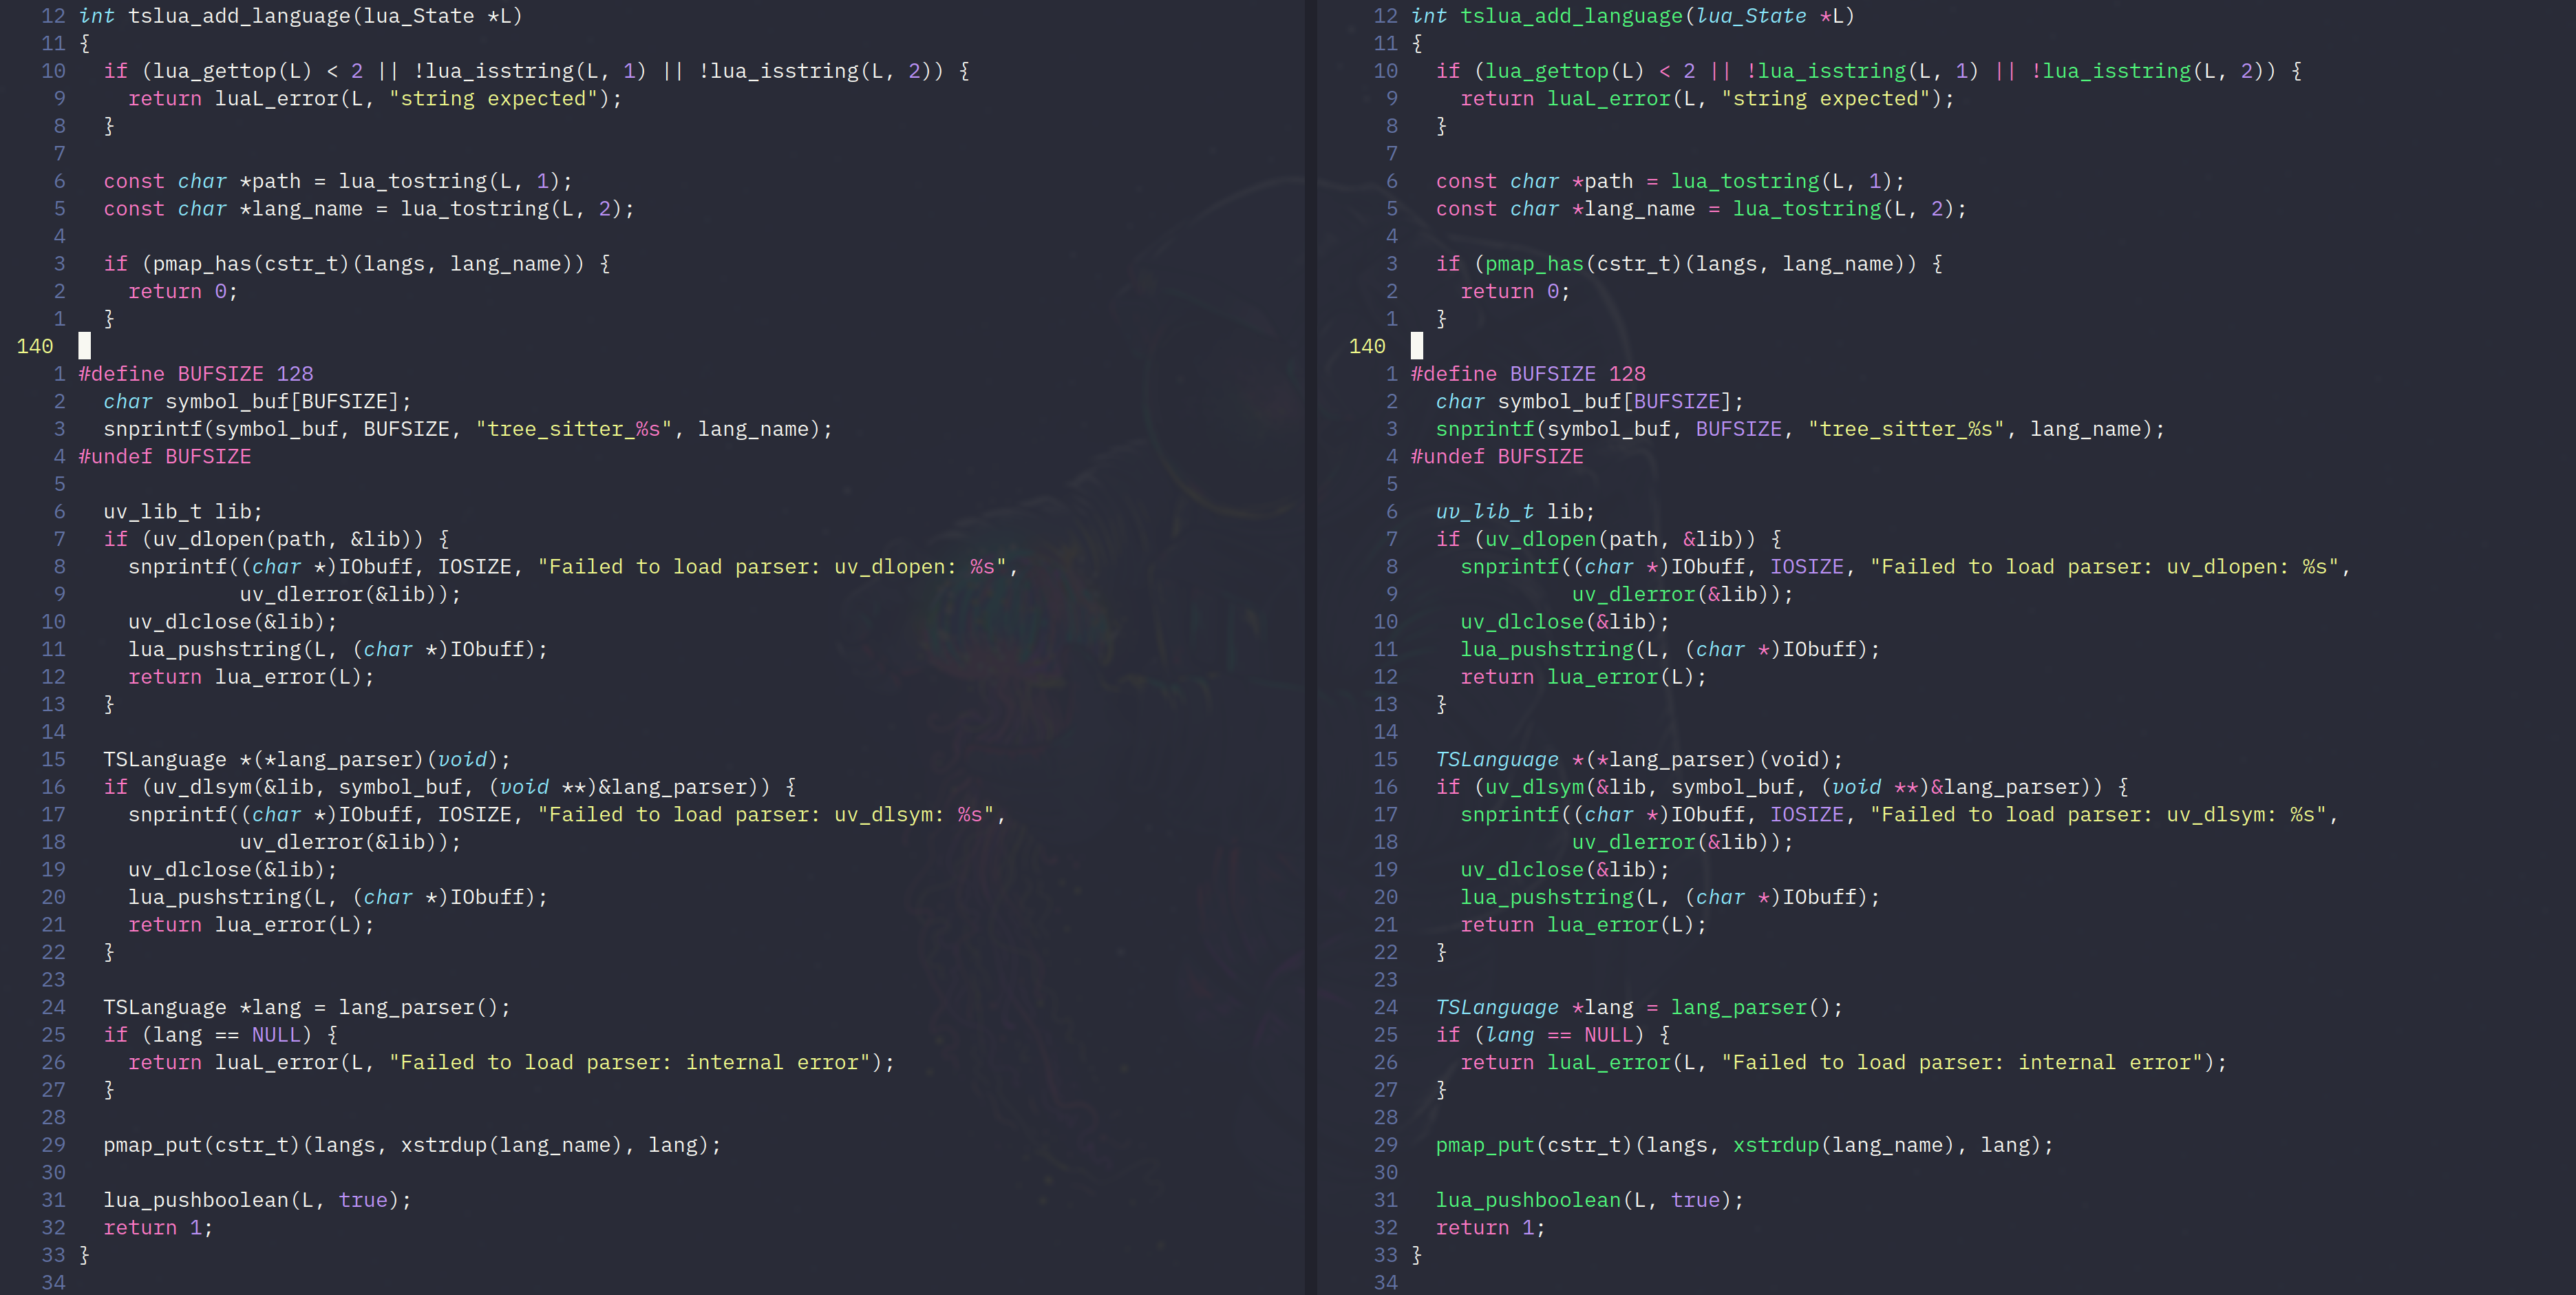
\includegraphics[width=0.6\linewidth]{./Figures/Treesitter_compare.png}
      \caption{使用Treesitter前 vs. 使用Treesitter后}%
    \end{figure}
  \end{frame}

  \begin{frame}{代码补全}{Language Server Protocol (LSP)}
    \link{语言服务器协议}{https://learn.microsoft.com/zh-cn/visualstudio/extensibility/language-server-protocol?view=vs-2022}(Language Server Protocol, LSP),是对开发工具与语言服务器进程之间交换的消息进行标准化的产物
    \vspace{-1em}
    \begin{columns}[t]
      \begin{column}{0.5\linewidth}
        \small
        \begin{itemize}
          \item LSP之前:各个IDE为支持的语言编写各自的补全引擎
            \begin{center}
              \begin{tikzpicture}
                \node (java) at (0,0) {
\includegraphics[height=0.5cm]{./Figures/Java_logo.pdf}};
                \node (cpp) at (1,0) {
\includegraphics[height=0.5cm]{./Figures/C++_logo.pdf}};
                \node (python) at (2,0) {
\includegraphics[height=0.5cm]{./Figures/Python_logo.png}};
                \node (idea) at (0,-1) {\href{www.jetbrains.com}{\includegraphics[height=0.5cm]{./Figures/IDEA_logo.pdf}}};
                \node (clion) at (1,-1) {\href{www.jetbrains.com}{\includegraphics[height=0.5cm]{./Figures/Clion_logo.pdf}}};
                \node (pycharm) at (2,-1) {\href{www.jetbrains.com}{\includegraphics[height=0.5cm]{./Figures/Pycharm_logo.pdf}}};

                \draw[->,thick] (java) -- (idea);
                \draw[->,thick] (cpp) -- (clion);
                \draw[->,thick] (python) -- (pycharm);
              \end{tikzpicture}
            \end{center}
          \item 缺点:IDE与语言强绑定
        \end{itemize}
      \end{column}
      \pause

      \begin{column}{0.5\linewidth}
        \small
        \begin{itemize}
          \item LSP之后:编辑器与语言服务器通讯,获取对应语言的补全
            \begin{center}
              \begin{tikzpicture}
                \node (java) at (0,0) {
\includegraphics[height=0.5cm]{./Figures/Java_logo.pdf}};
                \node (cpp) at (1,0) {
\includegraphics[height=0.5cm]{./Figures/C++_logo.pdf}};
                \node (python) at (2,0) {
\includegraphics[height=0.5cm]{./Figures/Python_logo.png}};

                \draw (0, -1) node [draw,align=center] (java_lsp) {\tiny Java\\[-0.5em] \tiny LSP};
                \draw (1, -1) node [draw,align=center] (cpp_lsp) {\tiny C++\\[-0.5em] \tiny LSP};
                \draw (2, -1) node [draw,align=center] (python_lsp) {\tiny Python\\[-0.5em] \tiny LSP};

                \node (vscode) at (0.5,-2) {\href{https://code.visualstudio.com/}{\includegraphics[height=0.5cm]{./Figures/Vscode_logo.pdf}}};
                \node (neovim) at (1.5,-2) {\href{https://neovim.io/}{
\includegraphics[height=0.5cm]{./Figures/Neovim_logo.png}}};

                \draw[->,thick] (java) -- (java_lsp);
                \draw[->,thick] (cpp) -- (cpp_lsp);
                \draw[->,thick] (python) -- (python_lsp);

                \draw[->,thick] (java_lsp.south) -- (vscode);
                \draw[->,thick] (cpp_lsp.south) -- (vscode);
                \draw[->,thick] (python_lsp.south) -- (vscode);

                \draw[->,thick] (java_lsp.south) -- (neovim);
                \draw[->,thick] (cpp_lsp.south) -- (neovim);
                \draw[->,thick] (python_lsp.south) -- (neovim);
              \end{tikzpicture}
            \end{center}
          \item 优点:编辑器与语言解耦
        \end{itemize}
      \end{column}
    \end{columns}

    \refnote{Copyright © 2025 JetBrains s.r.o. CLion, IDEA, and PyCharm \\[-0.7em] and the CLion, IDEA, and PyCharm logo are trademarks of JetBrains s.r.o.}
  \end{frame}

  \begin{frame}{代码补全}{补全引擎}

    \begin{columns}
      \begin{column}{0.5\linewidth}
        在Neovim中,需要通过一个补全引擎来将LSP提供的补全结果显示出来

        有多种补全引擎可供选择:
        \begin{itemize}
          \item \link{coc.nvim}{https://github.com/neoclide/coc.nvim}
          \item \link{mini.completion}{https://github.com/echasnovski/mini.completion}
          \item \link{nvim-cmp}{https://github.com/hrsh7th/nvim-cmp}
          \item \link{blink.cmp}{https://github.com/Saghen/blink.cmp} (我的选择)
        \end{itemize}

      \end{column}

      \begin{column}{0.5\linewidth}
        \begin{figure}[H]
          \centering
          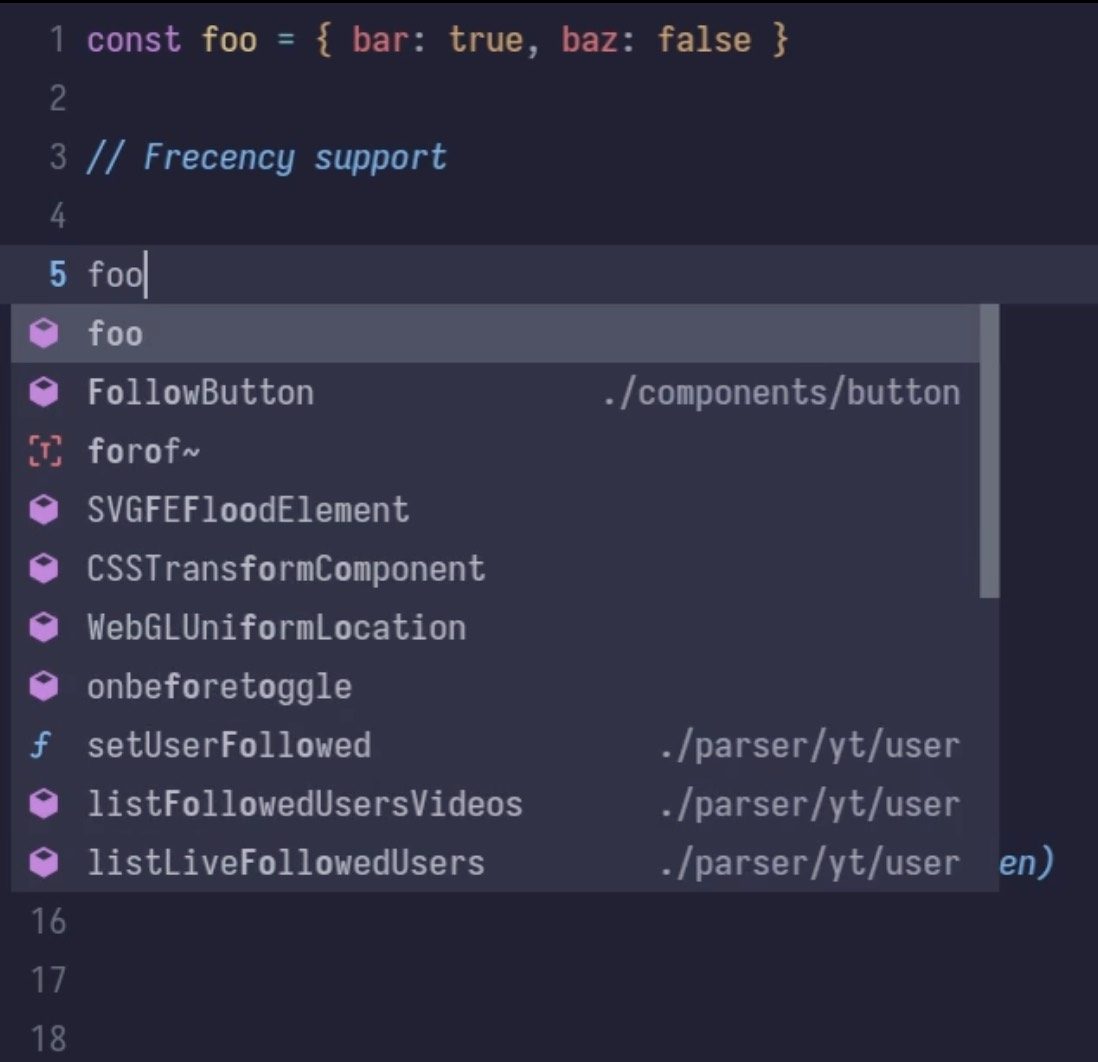
\includegraphics[width=0.8\textwidth]{./Figures/Completion_demo.jpg}
        \end{figure}

      \end{column}
    \end{columns}

  \end{frame}

\section{插件安装}
  \subsection{nvim-treesitter}
  \subsection{mason.nvim}
  \subsection{nvim-lspconfig}
  \subsection{blink.cmp}

    \begin{frame}{插件安装}
      \begin{itemize}
        \item \link{nvim-treesitter}{https://github.com/nvim-treesitter/nvim-treesitter}:语法高亮
        \item \link{mason.nvim}{https://github.com/williamboman/mason.nvim}:下载LSP
        \item \link{nvim-lspconfig}{https://github.com/neovim/nvim-lspconfig}:配置LSP
        \item \link{blink.cmp}{https://github.com/Saghen/blink.cmp}:代码补全引擎
      \end{itemize}
    \end{frame}

\section{插件配置}

  \begin{frame}{插件配置}
    \begin{itemize}
      \item nvim-treesitter:\lstinline[language={},style=path]{\~/.config/nvim/lua/plugins/treesitter.lua}
      \item mason.nvim:\lstinline[language={},style=path]{\~/.config/nvim/lua/plugins/lsp.lua}
      \item nvim-lspconfig:\lstinline[language={},style=path]{\~/.config/nvim/lua/plugins/lsp.lua}
      \item blink.cmp:\lstinline[language={},style=path]{\~/.config/nvim/lua/plugins/completion.lua}
    \end{itemize}
  \end{frame}

  \begin{frame}{Thanks}
    配色方案:
    \begin{itemize}
      \item \link{Catppuccin}{https://catppuccin.com/} 
\includegraphics[height=10pt]{./Figures/Catppuccin_logo.png}
      \item \link{Catppuccin for beamer}{https://github.com/atticus-sullivan/beamercolortheme}
    \end{itemize}
  \end{frame}

\end{document}
